    \documentclass[12pt,a4paper]{article}

    % ---------------------------------------------------------
    % Packages
    % ---------------------------------------------------------
    \usepackage[a4paper,
                left=1in,
                right=1in,
                top=0.8in,
                bottom=0.8in]{geometry}

    \usepackage{newtxtext}
    \usepackage{newtxmath}
    \usepackage{pgfgantt}
    \usepackage{graphicx}
    \usepackage{amssymb}
    \usepackage{array}
    \usepackage{tabularx}
    \usepackage{longtable}
    \usepackage{booktabs}
    \usepackage{multirow}
    \usepackage{enumitem}
    \usepackage{setspace}
    \usepackage{fancyhdr}
    \usepackage{titlesec}
    \usepackage{caption}
    \usepackage{subcaption}
    \usepackage{float}
    \usepackage{amssymb}
    \usepackage{pifont}
    \usepackage{ragged2e}
    \usepackage{url}
    \usepackage[hidelinks]{hyperref}
    \usepackage{xcolor}
    \usepackage{tikz}
    \usetikzlibrary{shapes.geometric, arrows.meta, positioning, fit, backgrounds, calc, decorations.markings}
    \usepackage{amsmath}
    \usepackage{colortbl}

    % ---------------------------------------------------------
    % Custom Colors
    % ---------------------------------------------------------
    \definecolor{darkblue}{RGB}{0,51,102}
    \definecolor{successgreen}{RGB}{34,139,34}
    \definecolor{warningred}{RGB}{178,34,34}

    % ---------------------------------------------------------
    % General Formatting
    % ---------------------------------------------------------
    \setlength{\parindent}{0pt}
    \setlength{\parskip}{6pt}

    \onehalfspacing

    % Section formatting
    \titleformat{\section}
    {\bfseries\large}
    {\thesection.}
    {0.5em}
    {}

    \titlespacing*{\section}
    {0pt}
    {12pt}
    {6pt}

    \titleformat{\subsection}
    {\bfseries\normalsize}
    {\thesubsection.}
    {0.5em}
    {}

    \titlespacing*{\subsection}
    {0pt}
    {8pt}
    {4pt}

    % ---------------------------------------------------------
    % Header / Footer
    % ---------------------------------------------------------
    \pagestyle{fancy}
    \fancyhf{}

    \fancyfoot[R]{\thepage\;|\;P a g e}

    \renewcommand{\headrulewidth}{0pt}
    \renewcommand{\footrulewidth}{0pt}

    % ---------------------------------------------------------
    % Table formatting
    % ---------------------------------------------------------
    \renewcommand{\arraystretch}{1.25}

    % ---------------------------------------------------------
    % Color definitions
    % ---------------------------------------------------------
    \definecolor{darkblue}{RGB}{0,51,102}
    \definecolor{lightgray}{RGB}{240,240,240}
    \definecolor{successgreen}{RGB}{34,139,34}
    \definecolor{warningred}{RGB}{178,34,34}

    % ---------------------------------------------------------
    % Custom commands
    % ---------------------------------------------------------

    % Green check mark similar to the original template
    \newcommand{\greencheck}{%
        \colorbox{green!50}{\Large\checkmark}%
    }

    % ---------------------------------------------------------
    % Document
    % ---------------------------------------------------------
    \begin{document}

    % =========================================================
    % COVER PAGE
    % =========================================================

    \begin{titlepage}
    \thispagestyle{empty}

    \begin{center}

    % ---------------------------------------------------------
    % University Logo
    % ---------------------------------------------------------

    \IfFileExists{vu_logo.png}{
        
\includegraphics[width=1.0in]{vu_logo.png}
        \vspace{0.2in}
    }{}

    {\Large\bfseries Varendra University}

    \vspace{0.08in}

    {\large\bfseries Department of Computer Science and Engineering}

    \vspace{0.55in}

    {\large\bfseries Undergraduate Thesis Proposal}

    \vspace{0.55in}

    {\large\bfseries Signal-Aware Machine Learning Calibration of a Low-Cost\\[4pt]
    Pan-Tilt Time-of-Flight LiDAR for Indoor 3D Reconstruction}

    \vfill

    {\bfseries Submitted by:}

    \vspace{0.25in}

    Oishi Farzana (232311294)\\
    Mahfuz Ahmad (232311307)\\
    Abdul Momit Talukder (232311320)

    \vspace{0.25in}

    \textbf{Program:} B.Sc. in Computer Science and Engineering\\
    \textbf{Semester:} 7th\\
    \textbf{Section:} E\\
    \textbf{Course Code:} CSE 4100\\
    \textbf{Course Title:} Project or Thesis with Seminar Part I

    \vfill

    {\bfseries Supervisor:}

    \vspace{0.08in}

    Mohd Ruhul Ameen\\
    Lecturer\\
    Department of Computer Science and Engineering

    \vfill

    {\bfseries Submission Date:} 07 October 2026

    \end{center}

    \end{titlepage}


    % =========================================================
    % TABLE OF CONTENTS
    % =========================================================

    \setcounter{page}{1}

    \tableofcontents
    \newpage


    % =========================================================
    % SECTION 1: INTRODUCTION
    % =========================================================

    \section{Introduction}

    Indoor three-dimensional (3D) mapping is a foundational capability for mobile robotics, autonomous navigation, augmented reality, structural inspection, and digital twin construction \cite{hess2016real, rusu20113d}. Commercial LiDAR systems---such as those manufactured by Velodyne, SICK, and Hokuyo---deliver high-resolution, dense point clouds with millimeter-level accuracy, but their costs typically range from \$500 to over \$10,000, rendering them impractical for educational laboratories, hobbyist robotics, and resource-constrained embedded applications in developing countries \cite{amann2001laser, behroozpour2017lidar}.

    A promising low-cost alternative is to mount a single-point Time-of-Flight (ToF) sensor on a two-axis pan-tilt mechanism using low-cost DC/N20 motors, sweeping it across the environment to collect one distance measurement at a time. Each measurement, combined with the corresponding pan and tilt angles, can be converted into a 3D Cartesian coordinate using the spherical-to-Cartesian transform. Thousands of such sequential measurements compose a 3D point cloud---a spatial representation of the scanned environment \cite{willis2009design, jimenez20143d}.

    The STMicroelectronics VL53L1X sensor is one of the most widely adopted single-point ToF sensors, integrating a 940\,nm VCSEL (Vertical-Cavity Surface-Emitting Laser) emitter, a 16$\times$16 SPAD (Single Photon Avalanche Diode) receiver array, and full timing/signal-processing logic into a single compact package costing approximately \$4 USD \cite{stmicro2018vl53l1x}. However, while the VL53L1X datasheet promises $\pm$3\% ranging accuracy under ideal conditions, real-world indoor scanning introduces systematic errors from multiple sources: multipath interference (MPI), target surface reflectivity variations, ambient light contamination, and mechanical jitter from low-cost pan-tilt actuators \cite{foix2011lock, hansard2012time, corti2016metrological}.

    This thesis proposes a \textbf{``Signal-Aware'' Machine Learning (ML) calibration} approach that exploits the sensor's internal photon telemetry---specifically, the signal return rate and ambient noise rate---as additional input features to a machine learning model that predicts and corrects measurement errors in real time. Critically, the trained model is transpiled into pure C code and deployed directly onto an ESP32 microcontroller, enabling real-time, on-device calibration without any external compute dependency. The entire hardware platform costs under \$22 USD, making it accessible for educational and research applications in resource-limited settings.

    Our work will further investigate the generalization of ML calibration across different indoor environments. We hypothesize that multi-environment pooled training will be important for robust performance, which will be investigated rigorously in the full study.


    % =========================================================
    % SECTION 2: LITERATURE REVIEW
    % =========================================================

    \section{Literature Review}

    \subsection{ToF Sensor Error Characterization}

    Time-of-Flight sensors compute distance by measuring the round-trip time of a modulated infrared laser pulse. The error characteristics of these sensors have been extensively studied. Corti et al. \cite{corti2016metrological} characterized the Kinect V2 ToF camera and found that measurement accuracy varies with temperature, range, surface properties, and radial position. Frangez et al. \cite{frangez2022assessment} demonstrated that ToF measurement accuracy varies with target distance, device temperature, and material properties, proposing improved calibration procedures. Kahlmann et al. \cite{kahlmann2006calibration} calibrated the SwissRanger camera, showing that systematic errors can be reduced through device-specific look-up tables. Lindner and Kolb \cite{lindner2006lateral} established foundational methods for combined geometric-radiometric correction of PMD sensors, while Fuchs and Hirzinger \cite{fuchs2008extrinsic} addressed extrinsic and depth calibration of ToF cameras.

    \subsection{Multipath Interference}

    Multipath interference (MPI) is one of the most significant error sources for ToF sensors operating in indoor environments. When emitted photons bounce off multiple surfaces before returning to the detector, the sensor averages arrival times from both direct and reflected paths, inflating the reported distance. Sabov and Kr\"uger \cite{sabov2008identification} proposed methods for identifying and correcting ``flying pixels'' caused by mixed-path returns at object boundaries. Reynolds et al. \cite{reynolds2011capturing} developed approaches for capturing ToF data with confidence measures, and Dorrington et al. \cite{dorrington2011separating} demonstrated techniques for separating true range from multi-path interference in commercial range cameras.

    \subsection{Machine Learning for Depth Correction}

    Recent works have demonstrated that ML models can effectively correct ToF measurement errors. Su et al. \cite{su2018deeptof} proposed DeepToF, showing that learned models can map complex ToF distortions to corrected depth maps. Agresti et al. \cite{agresti2018deep} showed that convolutional neural networks can exploit spatial context to reduce MPI artifacts. He et al. \cite{he2017depth} formalized residual error analysis for ToF cameras---a direct inspiration for our signal-aware approach. However, most existing approaches target imaging-class ToF cameras running on GPU-capable systems, leaving a gap for single-point sensors on microcontrollers.

    \subsection{Low-Cost LiDAR Systems}

    Several works have explored low-cost 3D scanning. Willis et al. \cite{willis2009design} presented an inexpensive LIDAR scanning system design. Jimenez et al. \cite{jimenez20143d} built a 3D scanner from a ToF camera and a pan-tilt unit. Kim and Lee \cite{kim2015design} designed and calibrated a pan-tilt ToF scanning system. Park et al. \cite{fpga2019lowcost} proposed an FPGA-based low-cost 3D LiDAR, and Low et al. \cite{low2024cost3d} developed a low-cost 3D mapping system using 2D LiDAR and monocular cameras. None of these works combine on-device ML calibration with signal telemetry features.

    \subsection{TinyML and Edge AI}

    The emerging field of TinyML focuses on deploying ML models on ultra-low-power microcontrollers \cite{warden2019tinyml, wang2020tinyml}. Hayajneh et al. \cite{hayajneh2024tinyml} demonstrated TinyML-empowered transfer learning on edge devices. Banbury et al. \cite{banbury2021benchmarking} established standardized benchmarks for TinyML systems. David et al. \cite{david2021tensorflow} presented TensorFlow Lite Micro for embedded ML, and Lin et al. \cite{lin2020mcunet} proposed MCUNet for tiny deep learning on IoT devices. Our work contributes to this field by demonstrating tree-model transpilation as a zero-dependency alternative to TFLite for sensor calibration on ESP32.

    \textbf{Research Gap:} While prior work has addressed ToF calibration using ML and has explored TinyML deployment independently, few existing works combine: (1) signal-telemetry-aware calibration of a single-point ToF sensor, (2) multi-environment generalization analysis, and (3) on-device model deployment via tree transpilation on a microcontroller---all within a sub-\$22 hardware platform.

    \subsection{Comparative Summary of Related Work}

    Table~\ref{tab:lit_comparison} summarizes key related works and identifies how each differs from our proposed approach.

    \begin{table}[H]
    \centering
    \caption{Comparative summary of related work.}
    \label{tab:lit_comparison}
    \small
    \begin{tabularx}{\textwidth}{|p{1.1in}|p{1.0in}|X|p{1.1in}|}
    \hline
    \textbf{Study} & \textbf{Sensor Type} & \textbf{Calibration Method} & \textbf{Limitation} \\
    \hline
    Kahlmann et al. \cite{kahlmann2006calibration} & SwissRanger (ToF camera) & Device-specific LUT & Single device, no ML \\
    \hline
    Su et al. \cite{su2018deeptof} & ToF camera & Deep learning (CNN) & Requires GPU inference \\
    \hline
    Agresti et al. \cite{agresti2018deep} & ToF camera & CNN for MPI removal & High compute cost \\
    \hline
    Kim \& Lee \cite{kim2015design} & Pan-tilt ToF & Geometric calibration & No ML, no telemetry \\
    \hline
    Lin et al. \cite{lin2020mcunet} & General MCU & TinyML (MCUNet) & Not applied to ToF \\
    \hline
    Willis et al. \cite{willis2009design} & Rotating LiDAR & Hardware design only & No calibration model \\
    \hline
    \textbf{Proposed Work} & \textbf{VL53L1X (single-point)} & \textbf{Signal-aware ML + tree transpilation on ESP32} & \textbf{Focuses on unseen room generalization} \\
    \hline
    \end{tabularx}
    \end{table}


    % =========================================================
    % SECTION 3: PROBLEM STATEMENT
    % =========================================================

    \section{Problem Statement}

    Low-cost ToF sensors such as the VL53L1X exhibit measurement errors that depend on multiple interacting variables: distance, scan angle, target surface reflectivity, ambient lighting conditions, and mechanical vibration. Traditional calibration methods employ polynomial look-up tables indexed solely by measured distance \cite{lindner2010time, kahlmann2006calibration}, assuming that range error is a one-dimensional function. This assumption is often insufficient in real scanning setups where error is a multi-dimensional function of the measurement context.

    Furthermore, existing ML-based depth correction approaches \cite{su2018deeptof, agresti2018deep, guo2021tackling} target imaging-class ToF cameras with GPU-based inference, and do not address single-point ToF sensors on resource-constrained microcontrollers. Even among low-cost LiDAR systems, none exploit the sensor's internal diagnostic telemetry (signal rate, ambient rate) as calibration features, and none evaluate whether ML calibration models generalize across different indoor environments.

    This thesis addresses the following core problem: \textit{Can the internal photon telemetry signals exposed by the VL53L1X sensor be leveraged by a machine learning model to predict and correct range measurement errors in real time on an ESP32 microcontroller, and can such calibration achieve held-out-room generalization across different indoor environments?}

    The problem is further compounded by the severe memory and compute constraints of the ESP32 platform (4\,MB flash, 520\,KB SRAM, 240\,MHz dual-core), which limits the size and complexity of deployable models.


    % =========================================================
    % SECTION 4: OBJECTIVES
    % =========================================================

    \section{Objectives}

    The following objectives are established for this thesis, aligned with SMART criteria:

    \begin{itemize}[leftmargin=0.35in]
        \item \textbf{Objective 1 (Hardware Platform) -- Target M4:} Design, assemble, and evaluate multiple functional 3D LiDAR scanning platforms by evaluating alternative pan-tilt mechanisms (e.g., DC gear motors, N20 motors, servos) and auxiliary sensing configurations around the VL53L1X to find the optimal balance of accuracy, power, and cost under \$25 USD.

        \item \textbf{Objective 2 (Data Collection) -- Target M8:} Collect a comprehensive dataset of over 150,000 ToF measurements across numerous diverse indoor and outdoor environments under challenging conditions (varied lighting, surface materials, dynamic obstacles).

        \item \textbf{Objective 3 (Signal-Aware ML Calibration) -- Target M9:} Train and evaluate machine learning models (Linear Regression, Random Forest, XGBoost, Gradient Boosting, MLP) that use both geometric features (distance, pan angle, tilt angle) and sensor telemetry features (signal rate, ambient rate, temperature) to predict and correct range measurement errors, targeting a Mean Absolute Error (MAE) below 25\,mm.

        \item \textbf{Objective 4 (Generalization Analysis) -- Target M10:} Quantify the cross-environment generalization performance of ML calibration models by evaluating single-environment models on unseen environments and comparing against multi-environment pooled training to establish held-out-room generalization.

        \item \textbf{Objective 5 (Edge Deployment) -- Target M11:} Deploy the trained calibration model onto the ESP32 microcontroller via model-to-C transpilation (m2cgen), achieving real-time inference (latency $<$ 100\,$\mu$s per prediction) with zero external dependencies and a code footprint $<$ 500\,KB.

        \item \textbf{Objective 6 (3D Reconstruction) -- Target M11:} Generate and visualize 3D point clouds from calibrated scan data, demonstrating improved spatial accuracy compared to raw sensor measurements.
    \end{itemize}


    % =========================================================
    % SECTION 5: RESEARCH QUESTIONS
    % =========================================================

    \section{Research Questions}

    This thesis seeks to answer the following core research questions:

    \begin{itemize}[leftmargin=0.35in]
        \item \textbf{RQ1:} To what extent can signal and ambient telemetry improve range-error prediction compared with geometry-only features?
        \item \textbf{RQ2:} How does calibration performance vary across indoor and outdoor environments?
        \item \textbf{RQ3:} Which ML model provides the best trade-off between calibration accuracy and embedded resource requirements?
        \item \textbf{RQ4:} Can the selected model operate in real time on an ESP32 without external inference dependencies?
    \end{itemize}


    % =========================================================
    % SECTION 5: PROPOSED METHODOLOGY / SYSTEM DESIGN
    % =========================================================

    \section{Proposed Methodology}

    \subsection{Overall System Architecture}

    The proposed system follows a five-stage pipeline: (1) hardware assembly and firmware development, (2) data collection across multiple environments, (3) ML model training and evaluation, (4) model transpilation and edge deployment, and (5) 3D point cloud reconstruction. Figure~\ref{fig:system_architecture} illustrates the end-to-end system architecture.

    \begin{figure}[H]
    \centering
    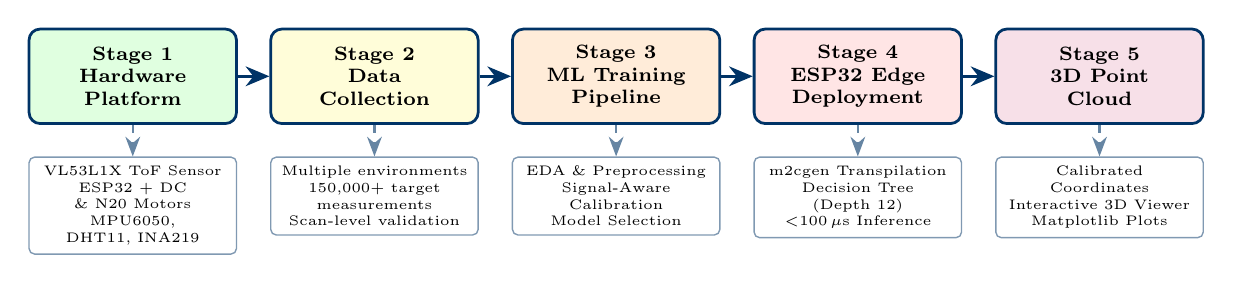
\begin{tikzpicture}[
        node distance=0.4cm,
        stage/.style={rectangle, draw=darkblue, fill=#1, text width=2.4cm, minimum height=1.2cm, align=center, rounded corners=4pt, font=\scriptsize\bfseries, line width=1pt},
        detail/.style={rectangle, draw=darkblue!50, fill=white, text width=2.4cm, minimum height=0.9cm, align=center, rounded corners=2pt, font=\tiny, line width=0.5pt},
        arrow/.style={-{Stealth[length=3mm, width=2.5mm]}, line width=1.2pt, darkblue},
        dasharrow/.style={-{Stealth[length=2.5mm]}, line width=0.8pt, darkblue!60, dashed}
    ]

    % Row 1: Main pipeline stages (evenly spaced)
    \node[stage=green!12] (hw) {Stage 1\\Hardware\\Platform};
    \node[stage=yellow!15, right=0.4cm of hw] (data) {Stage 2\\Data\\Collection};
    \node[stage=orange!15, right=0.4cm of data] (ml) {Stage 3\\ML Training\\Pipeline};
    \node[stage=red!10, right=0.4cm of ml] (deploy) {Stage 4\\ESP32 Edge\\Deployment};
    \node[stage=purple!12, right=0.4cm of deploy] (output) {Stage 5\\3D Point\\Cloud};

    % Row 2: Detail boxes (directly below each stage)
    \node[detail, below=0.4cm of hw] (hw_d) {VL53L1X ToF Sensor\\ESP32 + DC \& N20 Motors\\MPU6050, DHT11, INA219};
    \node[detail, below=0.4cm of data] (data_d) {Multiple environments\\150,000+ target measurements\\Scan-level validation};
    \node[detail, below=0.4cm of ml] (ml_d) {EDA \& Preprocessing\\Signal-Aware Calibration\\Model Selection};
    \node[detail, below=0.4cm of deploy] (deploy_d) {m2cgen Transpilation\\Decision Tree (Depth 12)\\$<$100\,$\mu$s Inference};
    \node[detail, below=0.4cm of output] (output_d) {Calibrated Coordinates\\Interactive 3D Viewer\\Matplotlib Plots};

    % Main pipeline arrows
    \draw[arrow] (hw) -- (data);
    \draw[arrow] (data) -- (ml);
    \draw[arrow] (ml) -- (deploy);
    \draw[arrow] (deploy) -- (output);

    % Stage-to-detail arrows
    \draw[dasharrow] (hw) -- (hw_d);
    \draw[dasharrow] (data) -- (data_d);
    \draw[dasharrow] (ml) -- (ml_d);
    \draw[dasharrow] (deploy) -- (deploy_d);
    \draw[dasharrow] (output) -- (output_d);

    \end{tikzpicture}
    \caption{End-to-end system architecture of the proposed Signal-Aware ML calibration pipeline.}
    \label{fig:system_architecture}
    \end{figure}


    \subsection{Hardware Design}

    The proposed scanning platform consists of nine components totaling under \$22 USD, as detailed in Table~\ref{tab:bom}. The VL53L1X ToF sensor will be mounted on a tilt motor, which is itself mounted on a pan motor, creating a two-axis gimbal. The sensor's optical center is positioned at the intersection of both rotation axes, defining the coordinate system origin $(0, 0, 0)$.

    \begin{table}[H]
    \centering
    \caption{Bill of Materials for the proposed scanning platform.}
    \label{tab:bom}
    \begin{tabularx}{\textwidth}{|p{1.5in}|p{1.3in}|X|p{0.5in}|}
    \hline
    \textbf{Component} & \textbf{Model} & \textbf{Role} & \textbf{Cost} \\
    \hline
    ToF Sensor & VL53L1X (I2C) & Distance measurement + signal telemetry & \$6 \\
    \hline
    Microcontroller & ESP32 DevKit V1 & Firmware, motor control, ML inference & \$4 \\
    \hline
    Pan Motor & 12V DC Gear Motor & Horizontal sweep 0\textdegree--180\textdegree & \$0.4 \\
    \hline
    Tilt Motor & N20 Motor & Vertical sweep 90\textdegree--180\textdegree & \$2 \\
    \hline
    Motor Driver & TB6612FNG & Motor speed and direction control & \$2 \\
    \hline
    3D Axis Monitor & MPU6050 (I2C) & Dual axis movement monitoring & \$2 \\
    \hline
    Temperature Sensor & DHT11 (GPIO 4) & Ambient thermal drift monitoring & \$1 \\
    \hline
    Current Monitor & INA219 (I2C) & Power consumption logging & \$2 \\
    \hline
    Power supply and others & Power supply and motor housing & Individual power to motors and sensors & \$2 \\
    \hline
    \multicolumn{3}{|r|}{\textbf{Total}} & \textbf{<\$22} \\
    \hline
    \end{tabularx}
    \end{table}

    Several actuator configurations (DC gear motors, N20 motors, servos) will be experimentally evaluated according to angular accuracy, repeatability, vibration, scanning speed, power consumption, and cost. The best-performing configuration will be selected for the final prototype.


    \subsection{Sensor Telemetry: The ``Signal-Aware'' Features}

    The key innovation of this work is the exploitation of the VL53L1X's internal diagnostic metrics as ML input features. Beyond the raw distance measurement, the sensor exposes two telemetry signals with every ranging cycle:

    \begin{itemize}[leftmargin=0.35in]
        \item \textbf{Signal Rate (kcps):} The strength of the reflected laser return, measured in kilo-counts per second. This metric serves as a proxy for target reflectivity and distance-dependent signal attenuation. Low signal rates indicate dark or distant targets where measurement noise is higher.
        \item \textbf{Ambient Rate (kcps):} The background infrared noise level detected by the SPAD array. This captures ambient lighting conditions---sunlight or strong room lighting degrades the signal-to-background ratio.
    \end{itemize}

    Our hypothesis is that these telemetry signals contain sufficient information about the physical state of the photon return to enable an ML model to predict \textit{why} the sensor is making a specific error and \textit{how much} to correct it.


    \subsection{Ground Truth Methodology}

    Since a reference-grade commercial LiDAR is not available, ground truth distances will be derived geometrically using ray-plane intersection:

    \begin{enumerate}[leftmargin=0.35in]
        \item The sensor's pan-tilt rotation center will be defined as the global origin $(0, 0, 0)$.
        \item A custom-printed protractor grid will be placed on the floor directly beneath the sensor, establishing angular reference lines every 5\textdegree~from 0\textdegree~to 180\textdegree.
        \item Target surfaces (walls, objects) will be measured with a tape measure ($\pm$1\,mm accuracy) at each 5\textdegree~pan interval.
        \item For intermediate pan angles, ground truth distances will be linearly interpolated.
        \item For non-horizontal tilt angles, a tilt correction will be applied based on the following geometric derivation.
    \end{enumerate}

    \textbf{Derivation of the tilt correction.} Consider the sensor at the origin emitting a beam toward a vertical wall at horizontal distance $d_h$. When the beam is horizontal ($\theta_{\text{tilt}} = 90^\circ$), it travels exactly $d_h$ to reach the wall. When the beam is tilted by an elevation angle $\alpha = |\theta_{\text{tilt}} - 90^\circ|$ from the horizontal plane, the beam must travel a longer slant path to intersect the same vertical wall plane. By basic trigonometry, the horizontal component of the slant distance $d$ equals $d \cos(\alpha) = d_h$, which gives:

    \begin{equation}
        d_{\text{GT}}(\theta_{\text{tilt}}) = \frac{d_{\text{GT, horizontal}}}{\cos(|\theta_{\text{tilt}} - 90^\circ|)}
        \label{eq:tilt_correction}
    \end{equation}

    This relation holds under the assumption that the target surface is a vertical plane perpendicular to the horizontal scan direction, which is valid for walls in typical indoor environments \cite{jimenez20143d, kim2015design}. Ground-truth uncertainty will be quantified and incorporated into the final error analysis.


    \subsection{Data Collection Strategy}

    To enable cross-environment analysis, data collection will be conducted across multiple indoor and outdoor environments. The initial data collection will include:

    \textbf{Environment 1 (Controlled Environment):} Proposed scanning sessions in a dark, controlled room with uniform painted walls. Pan range: 0\textdegree--180\textdegree~at 1\textdegree~steps; Tilt range: 90\textdegree--180\textdegree. This aims to collect approximately 50,000 trainable measurements (calculated across multiple environments $\times$ multiple sessions $\times$ pan angles $\times$ tilt angles $\times$ repeated scans).

    \textbf{Environment 2 (Diverse Environment):} Proposed scanning sessions under deliberately varied conditions to stress-test the sensor, as shown in Table~\ref{tab:day2_conditions}. The pan and tilt ranges will be identical to Environment 1.

    \begin{table}[H]
    \centering
    \caption{Proposed diverse scanning conditions designed to stress-test the sensor.}
    \label{tab:day2_conditions}
    \small
    \begin{tabularx}{\textwidth}{|c|p{1.2in}|p{0.8in}|X|}
    \hline
    \textbf{Scan} & \textbf{Condition} & \textbf{Lighting} & \textbf{Purpose} \\
    \hline
    1 & Dimmed lights & 50\% & Low-light performance \\
    \hline
    2 & Clean walls & Full bright & Bright baseline \\
    \hline
    3 & GT verification & Full bright & Cross-check measurements \\
    \hline
    4 & Mid-scan change & Mixed & Lighting transition handling \\
    \hline
    5 & Cardboard box & Full dark & Dark + obstacle detection \\
    \hline
    6 & Box + dark fabric & Full dark & Worst-case conditions \\
    \hline
    7 & Box + dark wall & Full bright & Challenging surfaces \\
    \hline
    8 & Box + covered wall & Full bright & Surface variation \\
    \hline
    9 & Dark wall only & Full bright & Low-reflectivity wall \\
    \hline
    10 & Transparent object & Full bright & Translucent material test \\
    \hline
    \end{tabularx}
    \end{table}


    \subsection{ML Problem Formulation}

    We formulate the calibration task as \textbf{residual error prediction}, following the residual error analysis framework established by He et al. \cite{he2017depth}. Given a raw sensor measurement $r_{\text{raw}}$ and the true distance $r_{\text{GT}}$, the residual error is defined as:

    \begin{equation}
        e = r_{\text{GT}} - r_{\text{raw}}
        \label{eq:residual}
    \end{equation}

    A positive $e$ indicates the sensor underestimates (reads short), while a negative $e$ indicates overestimation (reads long). The ML model $f(\mathbf{x})$ will learn to predict this residual from a 6-dimensional feature vector:

    \begin{equation}
        \hat{e} = f(\mathbf{x}), \quad \mathbf{x} = [r_{\text{raw}},\; \theta_{\text{pan}},\; \theta_{\text{tilt}},\; S_{\text{signal}},\; S_{\text{ambient}},\; T]
        \label{eq:feature_vector}
    \end{equation}

    where $S_{\text{signal}}$ is the signal rate (kcps), $S_{\text{ambient}}$ is the ambient noise rate (kcps), and $T$ is the ambient temperature (\textdegree C). The corrected distance follows directly from Eq.~\ref{eq:residual} by substituting the predicted residual $\hat{e}$ for the true residual $e$:

    \begin{equation}
        r_{\text{corrected}} = r_{\text{raw}} + \hat{e}
        \label{eq:correction}
    \end{equation}

    \textbf{Design Decision:} We propose predicting the \textit{residual error} rather than the absolute distance. Predicting distance directly often causes models to learn the identity function ($\hat{r} \approx r_{\text{raw}}$), ignoring all signal features. This observation is consistent with findings by He et al. \cite{he2017depth}, who showed that residual formulations are more effective for ToF error correction.

    Figure~\ref{fig:ml_pipeline} illustrates the complete ML training and inference pipeline.

    \begin{figure}[H]
    \centering
    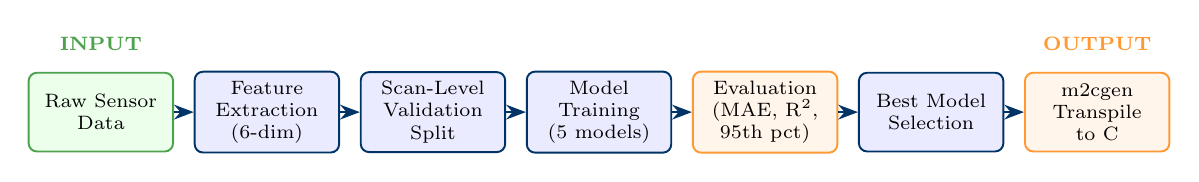
\begin{tikzpicture}[
        node distance=0.25cm,
        block/.style={rectangle, draw=darkblue, fill=blue!8, text width=1.6cm, minimum height=1.0cm, align=center, rounded corners=3pt, font=\scriptsize, line width=0.7pt},
        datablock/.style={rectangle, draw=successgreen!80, fill=green!8, text width=1.6cm, minimum height=1.0cm, align=center, rounded corners=3pt, font=\scriptsize, line width=0.7pt},
        resultblock/.style={rectangle, draw=orange!80, fill=orange!8, text width=1.6cm, minimum height=1.0cm, align=center, rounded corners=3pt, font=\scriptsize, line width=0.7pt},
        arrow/.style={-{Stealth[length=2.5mm]}, line width=0.8pt, darkblue}
    ]

    % Training Pipeline
    \node[datablock] (raw) {Raw Sensor\\Data};
    \node[block, right=0.25cm of raw] (feat) {Feature\\Extraction\\(6-dim)};
    \node[block, right=0.25cm of feat] (split) {Scan-Level\\Validation\\Split};
    \node[block, right=0.25cm of split] (train) {Model\\Training\\(5 models)};
    \node[resultblock, right=0.25cm of train] (eval) {Evaluation\\(MAE, R$^2$,\\95th pct)};
    \node[block, right=0.25cm of eval] (select) {Best Model\\Selection};
    \node[resultblock, right=0.25cm of select] (transpile) {m2cgen\\Transpile\\to C};

    % Arrows
    \draw[arrow] (raw) -- (feat);
    \draw[arrow] (feat) -- (split);
    \draw[arrow] (split) -- (train);
    \draw[arrow] (train) -- (eval);
    \draw[arrow] (eval) -- (select);
    \draw[arrow] (select) -- (transpile);

    % Labels
    \node[above=0.15cm of raw, font=\scriptsize\bfseries, text=successgreen!80] {INPUT};
    \node[above=0.15cm of transpile, font=\scriptsize\bfseries, text=orange!80] {OUTPUT};

    \end{tikzpicture}
    \caption{ML training pipeline: from raw sensor data to transpiled C code for ESP32 deployment.}
    \label{fig:ml_pipeline}
    \end{figure}


    \subsection{ML Models Evaluated}

    Five ML algorithms will be trained and compared across four training scenarios:

    \begin{table}[H]
    \centering
    \caption{ML models and their hyperparameters.}
    \label{tab:models}
    \begin{tabularx}{\textwidth}{|p{1.5in}|X|p{1.4in}|}
    \hline
    \textbf{Model} & \textbf{Description} & \textbf{Configuration} \\
    \hline
    Linear Regression & Baseline linear model & Default \\
    \hline
    Random Forest & Ensemble of decision trees with bagging & 100 trees, depth 12 \\
    \hline
    XGBoost & Gradient-boosted decision-tree model for nonlinear tabular regression & 200 trees, depth 8 \\
    \hline
    Gradient Boosting & Sklearn gradient boosting & 150 trees, depth 6 \\
    \hline
    MLP Neural Network & Multi-layer perceptron & 2 layers: 128, 64 \\
    \hline
    \end{tabularx}
    \end{table}

    Four training scenarios will be evaluated to study generalization:
    \begin{enumerate}[leftmargin=0.35in]
        \item \textbf{Single Environment:} scan-level 80/20 split
        \item \textbf{Forward Transfer:} train on Environment A, test on Environment B
        \item \textbf{Reverse Transfer:} train on Environment B, test on Environment A
        \item \textbf{Pooled Training:} scan-level 80/20 split across combined environments
    \end{enumerate}


    \subsection{Model Transpilation for ESP32 Deployment}

    For edge deployment, we will use the \texttt{m2cgen} (Model to C Code Generator) library to convert the selected sklearn model into a pure C function consisting entirely of nested if/else statements. The generated function signature will be:

    \begin{verbatim}
        double score(double * input);
    \end{verbatim}

    where \texttt{input} is a 6-element array containing the feature vector. This approach has \textbf{zero external dependencies}---no TensorFlow Lite, no ONNX runtime, no math libraries. The target is to achieve an inference latency below 100\,$\mu$s per prediction on the ESP32.

    Figure~\ref{fig:edge_deployment} illustrates the on-device inference cycle.

    \begin{figure}[H]
    \centering
    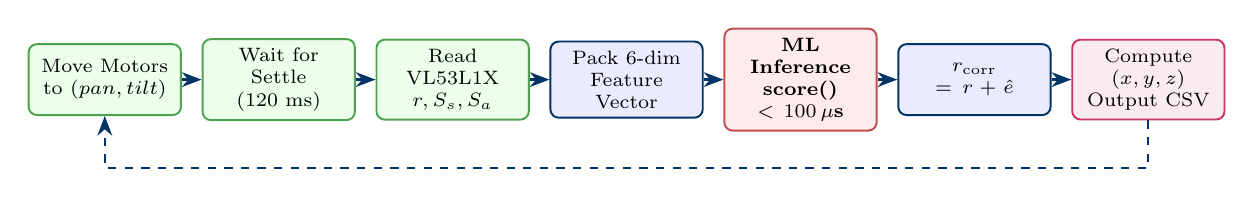
\begin{tikzpicture}[
        node distance=0.25cm,
        pstep/.style={rectangle, draw=darkblue, fill=blue!8, text width=1.7cm, minimum height=0.9cm, align=center, rounded corners=3pt, font=\scriptsize, line width=0.7pt},
        hw/.style={rectangle, draw=successgreen!80, fill=green!8, text width=1.7cm, minimum height=0.9cm, align=center, rounded corners=3pt, font=\scriptsize, line width=0.7pt},
        ml/.style={rectangle, draw=warningred!80, fill=red!8, text width=1.7cm, minimum height=0.9cm, align=center, rounded corners=3pt, font=\scriptsize\bfseries, line width=0.7pt},
        pout/.style={rectangle, draw=purple!80, fill=purple!8, text width=1.7cm, minimum height=0.9cm, align=center, rounded corners=3pt, font=\scriptsize, line width=0.7pt},
        arrow/.style={-{Stealth[length=2.5mm]}, line width=0.8pt, darkblue}
    ]

    \node[hw] (move) {Move Motors\\to $(pan, tilt)$};
    \node[hw, right=0.25cm of move] (settle) {Wait for\\Settle\\(120 ms)};
    \node[hw, right=0.25cm of settle] (read) {Read VL53L1X\\$r, S_s, S_a$};
    \node[pstep, right=0.25cm of read] (pack) {Pack 6-dim\\Feature\\Vector};
    \node[ml, right=0.25cm of pack] (infer) {ML Inference\\score()\\$< 100\,\mu$s};
    \node[pstep, right=0.25cm of infer] (correct) {$r_{\text{corr}}$\\$= r + \hat{e}$};
    \node[pout, right=0.25cm of correct] (xyz) {Compute\\$(x,y,z)$\\Output CSV};

    \draw[arrow] (move) -- (settle);
    \draw[arrow] (settle) -- (read);
    \draw[arrow] (read) -- (pack);
    \draw[arrow] (pack) -- (infer);
    \draw[arrow] (infer) -- (correct);
    \draw[arrow] (correct) -- (xyz);

    % Loop arrow
    \draw[arrow, dashed] (xyz.south) -- ++(0,-0.6) -| (move.south);

    \end{tikzpicture}
    \caption{On-device inference cycle on the ESP32: each scan point goes through ML correction in real time.}
    \label{fig:edge_deployment}
    \end{figure}


    \subsection{Spherical-to-Cartesian Transform}

    Each calibrated measurement will be converted to 3D Cartesian coordinates for point cloud reconstruction using the standard spherical-to-Cartesian coordinate transform \cite{hansard2012time, jimenez20143d}. In our coordinate convention, $\theta_{\text{pan}}$ is the azimuthal angle measured in the horizontal plane, and the elevation angle is $\phi = \theta_{\text{tilt}} - 90^\circ$ (measured from the horizontal). The standard spherical transform $(r, \theta, \phi) \rightarrow (x, y, z)$ gives:

    \begin{equation}
        \begin{bmatrix} x \\ y \\ z \end{bmatrix} =
        \begin{bmatrix}
            r_{\text{corr}} \cdot \cos(\theta_{\text{tilt}} - 90^\circ) \cdot \cos(\theta_{\text{pan}}) \\
            r_{\text{corr}} \cdot \cos(\theta_{\text{tilt}} - 90^\circ) \cdot \sin(\theta_{\text{pan}}) \\
            r_{\text{corr}} \cdot \sin(\theta_{\text{tilt}} - 90^\circ)
        \end{bmatrix}
        \label{eq:spherical}
    \end{equation}

    where $r_{\text{corr}}$ is the ML-calibrated range from Eq.~\ref{eq:correction}. This transform will be applied identically on the ESP32 during real-time scanning and in the post-processing Python pipeline.


    % =========================================================
    % SECTION 6: METHOD JUSTIFICATION
    % =========================================================

    \section{Method Justification}

    The proposed methodology is justified on several grounds:

    \textbf{1. Residual Prediction over Absolute Prediction:} Training the model to predict the residual error $e = r_{\text{GT}} - r_{\text{raw}}$ rather than the absolute distance prevents the model from learning the identity function. When trained to predict distance directly, the model simply echoes the raw distance and ignores signal features entirely. Residual formulation forces the model to learn the \textit{error structure}, which is where signal telemetry is most informative.

    \textbf{2. Tree-Based Models over Neural Networks:} Decision Trees and Random Forests transpile to pure C if/else statements with zero external dependencies. Neural networks would require TFLite Micro or custom fixed-point inference libraries, adding complexity and potential failure modes. Tree-based models will be investigated because their decision structure can be transpiled into lightweight C code, potentially enabling dependency-free inference on the ESP32 while maintaining acceptable predictive accuracy.

    \textbf{3. Signal-Aware Features:} The inclusion of signal rate, ambient rate, and temperature as features is justified by the physics of ToF measurement. Signal rate captures target reflectivity and MPI effects; ambient rate captures lighting conditions; temperature captures thermal drift. 
    \textbf{Planned Validation:} The proposed methodology will be evaluated experimentally through controlled data collection, feature ablation, cross-environment validation, and embedded deployment experiments.

    \textbf{4. Multi-Environment Training:} The study will investigate whether single-environment models overfit to environment-specific error patterns and whether pooled multi-environment training improves robustness to domain shift.

    \textbf{5. m2cgen Transpilation:} Unlike TFLite which requires quantization, model conversion, and a runtime interpreter, m2cgen produces a standalone C function that any C compiler can handle. This eliminates dependency management and reduces the risk of deployment failures on embedded platforms.

    \subsection{Component Selection Justification}

    Table~\ref{tab:component_justification} compares each selected component against realistic alternatives, justifying our design choices.

    \begin{table}[H]
    \centering
    \caption{Component selection justification against alternatives.}
    \label{tab:component_justification}
    \small
    \begin{tabularx}{\textwidth}{|p{0.8in}|p{1.0in}|p{1.0in}|X|}
    \hline
    \textbf{Category} & \textbf{Selected} & \textbf{Alternative} & \textbf{Justification} \\
    \hline
    ToF Sensor & VL53L1X & HC-SR04 (Ultrasonic) & VL53L1X provides diagnostic telemetry such as signal rate, ambient rate, and sigma; signal and ambient rates are used as calibration features in the current study. \\
    \hline
    MCU & ESP32 & Arduino Uno & ESP32 has 4\,MB flash (fits transpiled model), dual-core 240\,MHz, and native I2C/PWM; Arduino Uno has only 32\,KB flash \\
    \hline
    Pan/Tilt Motors & DC Gear \& N20 & SG90 Servo & DC Gear/N20 motors provide continuous rotation capability; SG90 servos are restricted to 180\textdegree~and introduce severe mechanical jitter during slow sweeps \\
    \hline
    ML Framework & scikit-learn + m2cgen & TensorFlow Lite & Tree transpilation produces zero-dependency C code; TFLite requires a runtime interpreter and quantization pipeline \\
    \hline
    Temp. Sensor & DHT11 & BME280 & DHT11 costs \$1 and is sufficient to flag thermal drift; BME280 is more precise but costs \$5+ \\
    \hline
    \end{tabularx}
    \end{table}


    % =========================================================
    % SECTION 7: EXPECTED OUTCOMES
    % =========================================================

    \section{Expected Outcomes}

    The following outcomes are expected from this thesis research:

    \begin{enumerate}[leftmargin=0.35in]
        \item \textbf{Functional Hardware Platform:} A fully operational, optimal low-cost 3D LiDAR scanner (<\$25) derived from testing multiple hardware combinations, capable of performing automated pan-tilt scans and producing structured CSV data with distance, angle, and telemetry fields.

        \item \textbf{Comprehensive Multi-Environment Dataset:} A dataset containing more than 150,000 measurements across numerous indoor and outdoor environments under diverse conditions, with paired ground truth distances. The target dataset size is derived from the planned number of environments, scanning sessions, angular positions, and repeated measurements. The project aims to release this dataset publicly for reproducibility.

        \item \textbf{Signal-Aware Calibration Evaluation:} Quantify the contribution of telemetry features by comparing geometry-only and signal-aware models using the corrected dataset.

        \item \textbf{Cross-Environment Generalization Analysis:} We expect pooled multi-environment training to achieve robust MAE reduction across unseen environments. Performance will be evaluated using scan-level validation.

        \item \textbf{ESP32 Edge Deployment:} A selected calibration model meeting the target latency and memory constraints will be deployed on the ESP32 for real-time inference. A Decision Tree will be evaluated as a strong candidate for this deployment.

        \item \textbf{3D Point Cloud Reconstruction:} Visual and quantitative evaluation of point-cloud quality---e.g., using plane-fitting RMSE for wall surfaces---after ML calibration.

        \item \textbf{Research Publication:} A research manuscript will be prepared based on the final findings and evaluated for submission to an appropriate conference or journal.
    \end{enumerate}


    % =========================================================
    % SECTION 8: TOOLS AND TECHNOLOGIES
    % =========================================================

    \section{Tools and Technologies to Be Used}

    \begin{table}[H]
    \centering
    \caption{Tools, technologies, and resources used in this project.}
    \label{tab:tools}
    \begin{tabularx}{\textwidth}{|p{1.2in}|X|}
    \hline
    \textbf{Category} & \textbf{Tools / Technologies} \\
    \hline
    \textbf{Hardware} & VL53L1X ToF sensor, ESP32 DevKit V1, pan-tilt motors (DC/N20), DHT11, INA219, MPU6050 \\
    \hline
    \textbf{Firmware} & Arduino IDE, PlatformIO, C/C++, ESP32 Arduino Core \\
    \hline
    \textbf{ML \& Data Science} & Python 3.x, scikit-learn \cite{pedregosa2011scikit}, XGBoost \cite{chen2016xgboost}, NumPy, Pandas, Matplotlib, Seaborn \\
    \hline
    \textbf{Model Export} & m2cgen (Model to C Code Generator) \\
    \hline
    \textbf{Visualization} & Matplotlib (3D scatter plots), custom WebGL point cloud viewer (HTML/JavaScript) \\
    \hline
    \textbf{Version Control} & Git, GitHub \\
    \hline
    \textbf{Documentation} & \LaTeX{} (Overleaf), IEEE conference template \\
    \hline
    \textbf{Serial Interface} & Python Tkinter (custom Scanner UI for data collection) \\
    \hline
    \textbf{Operating Systems} & Windows 10/11 (development), ESP32 bare-metal (deployment) \\
    \hline
    \end{tabularx}
    \end{table}


    % =========================================================
    % SECTION 9: REFERENCES
    % =========================================================

    \section{References}

    \renewcommand{\refname}{}
    \bibliographystyle{IEEEtran}
    \bibliography{references}


    % =========================================================
    % SECTION 10: WORK DIVISION
    % =========================================================

    \section{Work Division and Team Management}

    Table~\ref{tab:work-division} describes the task distribution among team members. All members contribute collaboratively, with specialized focus areas.

    \begin{table}[H]
    \centering
    \caption{Work Division and Team Management}
    \label{tab:work-division}
    \begin{tabularx}{\textwidth}{|>{\raggedright\arraybackslash}p{1.6in}|X|>{\raggedright\arraybackslash}p{1.3in}|}
    \hline
    \textbf{Team Member} &
    \textbf{Assigned Tasks} &
    \textbf{Role} \\
    \hline

    Abdul Momit Talukder\newline (232311320) &
    Hardware assembly and integration, pan-tilt actuator calibration against protractor reference angles, physical preparation of indoor scanning environments, ground truth measurement, data collection campaigns, ESP32 deployment and testing, performance evaluation, and presentation preparation &
    Team Leader \& Hardware Engineer \\
    \hline

    Mahfuz Ahmad\newline (232311307) &
    Firmware development (data collection \& inference), ground truth measurement, ML pipeline design and model training, tool development (protractor generator, scanner UI), data collection and scanning, m2cgen model transpilation, ESP32 deployment, and point cloud visualization &
    Software Developer \& ML Engineer \\
    \hline

    Oishi Farzana\newline (232311294) &
    Literature review and research gap identification, exploratory data analysis (EDA), data preprocessing, result interpretation and comparative analysis, thesis writing and documentation, reference management, paper formatting, and presentation slide preparation &
    Researcher \& Technical Writer \\
    \hline

    \end{tabularx}
    \end{table}


    % =========================================================
    % SECTION 11: TIMELINE
    % =========================================================

    \section{Timeline}

    The thesis spans two semesters: the 7th semester (6 months, M1--M6) and the 8th semester (6 months, M7--M12), totaling 12 months. The work will focus on evaluating combinations of sensors and motors, developing the final optimized platform, executing large-scale data collection across environments, and conducting cross-environment generalization studies. Figure~\ref{fig:thesis_timeline} presents the complete proposed timeline.

    \begin{figure}[H]
    \centering
    \resizebox{\textwidth}{!}{%
    \begin{ganttchart}[
        hgrid,
        vgrid,
        x unit=1.0cm,
        y unit title=0.7cm,
        y unit chart=0.6cm,
        title height=1,
        bar height=0.5,
        bar label font=\small,
        title label font=\small\bfseries,
        bar/.append style={fill=blue!25}
    ]{1}{12}

    \gantttitle{7th Semester}{6}
    \gantttitle{8th Semester}{6} \\

    \gantttitle{M1}{1}
    \gantttitle{M2}{1}
    \gantttitle{M3}{1}
    \gantttitle{M4}{1}
    \gantttitle{M5}{1}
    \gantttitle{M6}{1}
    \gantttitle{M7}{1}
    \gantttitle{M8}{1}
    \gantttitle{M9}{1}
    \gantttitle{M10}{1}
    \gantttitle{M11}{1}
    \gantttitle{M12}{1} \\

    % --- Phase 1: Foundation (M1-M3) ---
    \ganttbar{Literature Review \& Gap Analysis}{1}{2} \\
    \ganttbar{Initial Hardware Prototyping}{1}{1} \\
    \ganttbar{Firmware Development}{1}{2} \\
    \ganttbar{Initial Setup \& Testing}{2}{3} \\
    \ganttbar{Baseline ML Pipeline Setup}{2}{3} \\
    % --- Remaining 7th Semester (M4-M6) ---
    \ganttbar{Hardware Combinations Assembly \& Testing}{4}{4} \\
    \ganttbar{Large-Scale Data Collection (Indoor/Outdoor)}{4}{5} \\
    \ganttbar{Final Model Training \& Feature Ablation}{5}{5} \\
    \ganttbar{3D Point Cloud Visualization}{5}{6} \\
    \ganttbar{Proposal Presentation}{6}{6} \\
    % --- 8th Semester (M7-M12) ---
    \ganttbar{3rd Environment Data Collection}{7}{8} \\
    \ganttbar{Outdoor / Adversarial Testing}{8}{9} \\
    \ganttbar{Model Generalization Study}{9}{10} \\
    \ganttbar{Research Paper Finalization}{9}{11} \\
    \ganttbar{Thesis Document Writing}{8}{11} \\
    \ganttbar{Final Review \& Revision}{11}{12} \\
    \ganttbar{Thesis Defense}{12}{12}

    \end{ganttchart}%
    }
    \caption{Proposed 12-month thesis timeline across 7th and 8th semesters. All activities shown in the timeline are proposed/planned activities.}
    \label{fig:thesis_timeline}
    \end{figure}


    % =========================================================
    % SECTION 12: COST-BENEFIT ANALYSIS
    % =========================================================

    \section{Cost-Benefit Analysis}

    \begin{table}[H]
    \centering
    \caption{Cost-Benefit Analysis for the Proposed System.}
    \label{tab:cost_benefit}
    \begin{tabularx}{\textwidth}{|p{1.5in}|X|p{1.0in}|}
    \hline
    \textbf{Item} & \textbf{Description} & \textbf{Cost} \\
    \hline
    VL53L1X ToF Sensor & Primary sensing element (I2C) & \$6 \\
    \hline
    ESP32 DevKit V1 & Microcontroller for control and ML inference & \$4 \\
    \hline
    DC Gear \& N20 Motors & Pan and tilt actuation & \$2.4 \\
    \hline
    TB6612FNG & Motor Driver & \$2 \\
    \hline
    MPU6050, DHT11, INA219 & Axis, environmental, and power monitoring & \$5 \\
    \hline
    Power supply \& housing & Power delivery and mounting & \$2 \\
    \hline
    \textbf{Hardware Total} & & \textbf{<\$22 ($\approx$2,610 BDT)} \\
    \hline
    \hline
    Software Tools & Python, scikit-learn, Arduino IDE, Git & Free (OSS) \\
    \hline
    Overleaf & LaTeX document preparation & Free tier \\
    \hline
    \textbf{Software Total} & & \textbf{\$0} \\
    \hline
    \hline
    \multicolumn{2}{|r|}{\textbf{Grand Total}} & \textbf{<\$22 ($\approx$2,610 BDT)} \\
    \hline
    \end{tabularx}
    \end{table}

    \textbf{Benefit Analysis:} Commercial LiDAR systems cost \$500--\$10,000+. The proposed platform targets a hardware cost below \$22 ($\approx$2,610 BDT), substantially lower than commercially available 3D sensing systems. We aim to achieve functional 3D point cloud generation with an ML-calibrated accuracy target of $\sim$25\,mm MAE. Table~\ref{tab:economic_comparison} presents a direct economic comparison.

    \begin{table}[H]
    \centering
    \caption{Economic comparison with commercial LiDAR systems.}
    \label{tab:economic_comparison}
    \small
    \begin{tabularx}{\textwidth}{|X|c|c|c|}
    \hline
    \textbf{System} & \textbf{Approx. Cost} & \textbf{Typical Accuracy} & \textbf{On-Device ML} \\
    \hline
    Velodyne VLP-16 & \$4,000+ & $\pm$3 cm & No \\
    \hline
    Hokuyo URG-04LX & \$1,000+ & $\pm$3 cm (2D only) & No \\
    \hline
    RPLIDAR A1 & \$100+ & $\pm$5 cm (2D only) & No \\
    \hline
    Intel RealSense L515 & \$350+ & $\pm$5 mm (short range) & No \\
    \hline
    \textbf{Proposed Low-Cost Prototype} & \textbf{<\$22} & \textbf{Target: $\sim$25 mm MAE} & \textbf{Yes} \\
    \hline
    \end{tabularx}
    \end{table}

    The open-source nature of all software tools ensures zero recurring costs. The system is particularly valuable for:
    \begin{itemize}[leftmargin=0.35in]
        \item Educational institutions in developing countries with limited equipment budgets
        \item Hobbyist robotics projects requiring basic spatial awareness
        \item Research prototyping where cost-effective validation of concepts is needed before investing in commercial hardware
    \end{itemize}


    % =========================================================
    % SECTION 13: CONSTRAINTS AND LIMITATIONS
    % =========================================================

    \section{Constraints and Limitations}

    \begin{enumerate}[leftmargin=0.35in]
        \item \textbf{Environmental Constraint:} Evaluating the model's performance on a completely unseen environment is critical and will be a major focus of the generalization study to ensure it does not overfit to a specific room.

        \item \textbf{Data Logging Risks:} Synchronizing and reliably logging data from the VL53L1X, motors, and telemetry sensors at high speeds poses a risk of data corruption or dropped frames, requiring robust firmware design.

        \item \textbf{Ground Truth Accuracy:} Geometric ground truth methodology relying on manual wall measurements assumes empty spaces. Scanning objects (like boxes) will introduce complex ground truth modeling challenges that will require object-aware methodologies.

        \item \textbf{Generalization vs. Memorization:} There is a risk that models might memorize room geometry (e.g., pan angles) rather than learning physical error relationships. Mitigating this will require careful train-test splits, such as leave-one-scan-out cross-validation across multiple environments.
    \end{enumerate}


    % =========================================================
    % SECTION 14: SOCIETAL IMPACT
    % =========================================================

    \section{Societal Impact}

    This thesis contributes to society in several meaningful ways:

    \textbf{Democratizing 3D Sensing Technology:} By reducing the core hardware cost to below \$22, this work makes spatial sensing technology accessible to students, educators, and researchers in developing countries who cannot afford commercial systems. This directly supports digital inclusion and STEM education.

    \textbf{Advancing Edge AI for IoT:} The demonstration of on-device ML inference on a low-cost ESP32 microcontroller establishes a practical template for deploying intelligent sensor processing in resource-constrained IoT devices. The proposed technology may have future applications in smart agriculture, environmental monitoring, and low-cost infrastructure inspection.

    \textbf{Open-Source Contribution:} All firmware, ML pipeline code, and the research paper will be made publicly available via GitHub \newline (\url{https://github.com/Mr-Mahfuz/signal-aware-tof-calibration}), enabling other researchers to reproduce, extend, and build upon this work.

    \textbf{Assistive Technology Potential:} Low-cost 3D spatial awareness has the potential to enable future applications such as assistive navigation devices for visually impaired individuals, obstacle detection for small autonomous vehicles, and affordable structural monitoring for buildings in earthquake-prone regions.

    \textbf{Educational Value:} The end-to-end nature of this project---spanning hardware design, firmware programming, data science, ML model training, embedded deployment, and scientific writing---provides a comprehensive learning experience that develops multiple engineering competencies simultaneously.


    % =========================================================
    % SECTION 15: COMPLEX ENGINEERING PROBLEM MAPPING
    % =========================================================

    \section{Complex Engineering Problem Mapping}

    Table~\ref{tab:complex-problem} maps the thesis to the complex engineering problem attributes defined by the accreditation framework.

    \begin{table}[H]
    \centering
    \caption{Mapping with complex problem solving.}
    \label{tab:complex-problem}

    \small
    \renewcommand{\arraystretch}{1.3}

    \begin{tabularx}{\textwidth}{|
    >{\centering\arraybackslash}X|
    >{\centering\arraybackslash}X|
    >{\centering\arraybackslash}X|
    >{\centering\arraybackslash}X|
    >{\centering\arraybackslash}X|
    >{\centering\arraybackslash}X|
    >{\centering\arraybackslash}X|}
    \hline

    \textbf{WP1} &
    \textbf{WP2} &
    \textbf{WP3} &
    \textbf{WP4} &
    \textbf{WP5} &
    \textbf{WP6} &
    \textbf{WP7} \\
    \hline

    Depth of Knowledge &
    Range of Conflicting Requirements &
    Depth of Analysis &
    Familiarity of Issues &
    Extent of Applicable Codes &
    Extent of Stakeholder Involvement &
    Inter\-dependence \\
    \hline

    {\Large\checkmark} &
    {\Large\checkmark} &
    {\Large\checkmark} &
    {\Large\checkmark} &
    &
    &
    \\
    \hline

    \end{tabularx}
    \end{table}

    \textbf{Justification:}
    \begin{itemize}[leftmargin=0.35in]
        \item \textbf{WP1 (Depth of Knowledge):} Requires deep understanding of ToF physics, ML algorithms, embedded systems, and signal processing---spanning multiple engineering disciplines.
        \item \textbf{WP2 (Conflicting Requirements):} The tension between model accuracy and memory footprint (e.g., large ensemble models vs. lightweight Decision Trees) exemplifies conflicting design requirements for embedded deployment.
        \item \textbf{WP3 (Depth of Analysis):} Involves statistical analysis (MAE, R$^2$, 95th percentile), cross-environment transfer studies, feature ablation, and model size sweeps.
        \item \textbf{WP4 (Familiarity of Issues):} Combining TinyML with ToF sensor calibration is an emerging, unfamiliar problem domain without established solutions.
    \end{itemize}


    % =========================================================
    % SECTION 16: COMPLEX ENGINEERING ACTIVITY MAPPING
    % =========================================================

    \section{Complex Engineering Activity Mapping}

    \begin{table}[H]
    \centering
    \caption{Mapping with complex engineering activities.}
    \label{tab:complex-activity}

    \small
    \renewcommand{\arraystretch}{1.3}

    \begin{tabularx}{\textwidth}{|
    >{\centering\arraybackslash}X|
    >{\centering\arraybackslash}X|
    >{\centering\arraybackslash}X|
    >{\centering\arraybackslash}X|
    >{\centering\arraybackslash}X|}
    \hline

    \textbf{EA1} &
    \textbf{EA2} &
    \textbf{EA3} &
    \textbf{EA4} &
    \textbf{EA5} \\
    \hline

    Range of resources &
    Level of Interaction &
    Innovation &
    Consequences for society and environment &
    Familiarity \\
    \hline

    {\Large\checkmark} &
    {\Large\checkmark} &
    &
    &
    \\
    \hline

    \end{tabularx}
    \end{table}

    \textbf{Justification:}
    \begin{itemize}[leftmargin=0.35in]
        \item \textbf{EA1 (Range of Resources):} Utilizes diverse resources: electronic hardware, firmware programming, Python data science libraries, embedded C, LaTeX, and version control systems.
        \item \textbf{EA2 (Level of Interaction):} The system involves complex interaction between optical sensing (photon physics), mechanical actuation (motor control), digital signal processing, and statistical learning.
    \end{itemize}


    % =========================================================
    % SECTION 17: GREEN COMPUTING
    % =========================================================

    \section{Green Computing Considerations}

    This thesis actively incorporates green computing principles:

    \begin{itemize}[leftmargin=0.35in]
        \item \textbf{Ultra-Low Power Deployment:} Power consumption will be measured using the INA219 to evaluate the energy cost of scanning and on-device inference.

        \item \textbf{Zero-Dependency Inference:} By transpiling the model to pure C code (no TFLite runtime, no ONNX interpreter), we eliminate unnecessary software bloat and reduce the computational overhead of inference.

        \item \textbf{Local Processing:} All inference occurs on-device. There is no need for cloud connectivity, eliminating data transmission energy costs and cloud server power consumption.

        \item \textbf{Hardware Minimalism:} The entire system uses multiple commodity components (under \$25 total). No custom PCB fabrication, no specialized manufacturing, and minimal electronic waste.

        \item \textbf{Open-Source Software:} All tools used (Python, scikit-learn, Arduino) are open-source, requiring no proprietary server infrastructure or licensing energy overhead.

        \item \textbf{Reusable Hardware:} All components are standard hobbyist parts that can be repurposed for other projects after the thesis is complete, minimizing e-waste.
    \end{itemize}


    % =========================================================
    % SECTION 18: LIFELONG LEARNING
    % =========================================================

    \section{Lifelong Learning and Personal Development}

    This thesis project contributes substantially to the team members' long-term professional development across multiple engineering domains:

    \begin{itemize}[leftmargin=0.35in]
        \item \textbf{Embedded Systems Engineering:} Hands-on experience with microcontroller programming, I2C communication, PWM motor control, and hardware debugging develops practical embedded systems skills directly applicable to IoT and robotics careers.

        \item \textbf{Machine Learning Engineering:} End-to-end ML pipeline experience---from data collection and EDA through model training, evaluation, and deployment---builds foundational ML engineering competence.

        \item \textbf{TinyML and Edge AI:} Working with model transpilation and resource-constrained deployment develops specialized skills in the rapidly growing TinyML field, which is projected to become a multi-billion-dollar industry.

        \item \textbf{Scientific Research Methodology:} Formulating hypotheses, designing controlled experiments, performing statistical analysis, writing reproducible research papers, and honestly reporting limitations develops rigorous scientific thinking.

        \item \textbf{Cross-Disciplinary Integration:} The project spans optics (ToF physics), mechanical engineering (motor systems), computer science (ML, firmware), and statistics (evaluation metrics), developing the ability to work across traditional disciplinary boundaries.

        \item \textbf{Technical Communication:} Writing LaTeX documents, creating scientific figures, and presenting quantitative results develops technical writing and presentation skills essential for any engineering career.

        \item \textbf{Version Control and Collaboration:} Using Git/GitHub for collaborative development builds software engineering best practices that are industry-standard.
    \end{itemize}


    \end{document}
